\documentclass[12pt,a4paper,titlepage,final]{article}

% cestina a fonty
\usepackage[czech]{babel}
\usepackage[utf8]{inputenc}
% balicky pro odkazy
\usepackage[bookmarksopen,colorlinks,plainpages=false,urlcolor=blue,unicode]{hyperref}
\usepackage{url}
% obrazky
\usepackage[dvipdf]{graphicx}
% velikost stranky
\usepackage[top=3.5cm, left=2.5cm, text={17cm, 24cm}, ignorefoot]{geometry}


\begin{document}

%%%%%%%%%%%%%%%%%%%%%%%%%%%%%%%%%%%%%%%%%%%%%%%%%%%%%%%%%%%%%%%%%%%%%%%%%%%%%%%%

	% titulní strana

	\def\author{Roman Blanco}
	\def\email{xblanc01@stud.fit.vutbr.cz}
	\def\projname{Semestrální projekt}

	\begin{titlepage}

	% \vspace*{1cm}
	\begin{figure}[!h]
	  \centering
	  
\includegraphics[height=5cm]{img/logo.eps}
	\end{figure}

	\vfill

	\begin{center}
		\begin{Large}
			ITO - Teorie obvodů\\
		\end{Large}
		\bigskip
			\begin{Huge}
				\projname\\
			\end{Huge}
		\begin{large}
			Řešení zadaných obvodů
		\end{large}
	\end{center}

	\vfill

	\begin{center}
		\begin{Large}
			\today
		\end{Large}
	\end{center}

	\vfill

	\begin{flushleft}
		\begin{large}
			\begin{tabular}{ll}
			Autor: & \author, \url{\email} \\
			 & Fakulta Informačních Technologií \\
			 & Vysoké Učení Technické v~Brně \\
			\end{tabular}
		\end{large}
	\end{flushleft}
\end{titlepage}


%%%%%%%%%%%%%%%%%%%%%%%%%%%%%%%%%%%%%%%%%%%%%%%%%%%%%%%%%%%%%%%%%%%%%%%%%%%%%%%%

% textova zprava

	\newpage
	\pagestyle{plain}
	\pagenumbering{arabic}
	\setcounter{page}{2}

%%%%%%%%%%%%%%%%%%%%%%%%%%%%%%%%%%%%%%%%%%%%%%%%%%%%%%%%%%%%%%%%%%%%%%%%%%%%%%%%

	\section*{Příklad č. 1 [A]} \label{pr1}

%===============================================================================

	\subsection*{Zadání}

	Stanovte napětí $U_{R_{7}}$ a proud $I_{R_{7}}$. Použíjte metodu
	postupného zjednodušování obvodu. \\

	\begin{minipage}[c]{0.5\textwidth}
		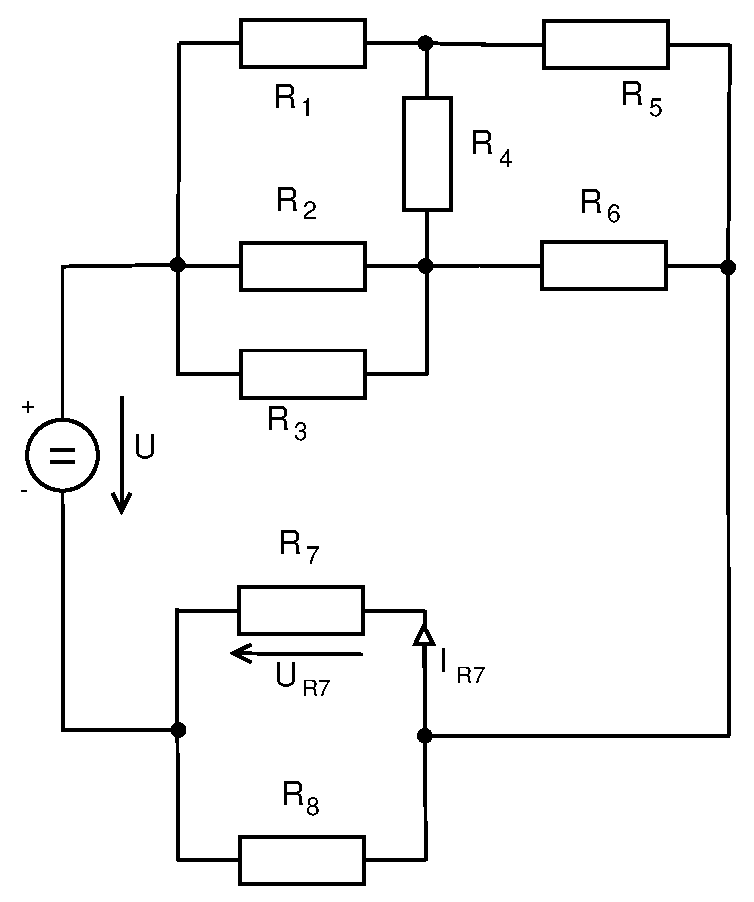
\includegraphics[height=7cm]{img/Pr1_2012.eps}
		\label{fig:pr1_obvod}
	\end{minipage}
	\begin{minipage}[c]{0.25\textwidth}
		$U = 80 V$ \\
		$R_{1} = 350 \Omega$ \\
		$R_{2} = 650 \Omega$ \\
		$R_{3} = 410 \Omega$ \\
		$R_{4} = 130 \Omega$ \\
		$R_{5} = 360 \Omega$ \\
		$R_{6} = 750 \Omega$ \\
		$R_{7} = 310 \Omega$ \\
		$R_{8} = 190 \Omega$ \\
		\\
		$U_{R_{7}} = ? V$ \\
		$I_{R_{7}} = ? A$
	\end{minipage}
	\\

%===============================================================================

	\subsection*{Výpočet}
	
	\quad Vypočítání paralelních obvodů: \\
	
	\begin{tabbing}
		$ { \displaystyle R_{78} = \frac{R_{7} \times R_{8}}
		{R_{7} + R_{8}} = 
		\frac{310 \times 190}{310 + 190} = 
		\frac{58900}{500} = 117,8 \Omega }$ \\
		\\
		$ { \displaystyle R_{23} = \frac{R_{2} \times R_{3}}
		{R_{2} + R_{3}} =
		\frac{650 \times 410}{650 + 410} =
		\frac{266500}{1060} = 251,4150943 \Omega} $ \\
	\end{tabbing}
	
	Konverze trojúhelníku na hvězdu: \\
	
	\begin{tabbing}
		$ { \displaystyle R_{A} = \frac{R_{1} \times R_{23}} 
		{R_{1} + R_{23} + R_{4}} = 
		\frac{87995,28301}{731,4150943} = 120,3082678 \Omega}$ \\
		\\
		$ { \displaystyle R_{B} = \frac{R_{1} \times R_{4}} 
		{R_{1} + R_{23} + R_{4}} = 
		\frac{45500}{731,4150943} = 62,20817748 \Omega}$ \\
		\\
		$ { \displaystyle R_{C} = \frac{R_{4} \times R_{23}} 
		{R_{1} + R_{23} + R_{4}} = 
		\frac{32683,96226}{731,4150943} = 44,68592802 \Omega}$ \\
	\end{tabbing}
	\newpage
	Vypočítání sériového zapojení obvodu ve stejných větvích: \\
	
	\begin{tabbing}
		$ { \displaystyle R_{B5} = R_{B} + R_{5} =
		404,68592802 \Omega }$ \\
		\\
		$ { \displaystyle R_{C6} = R_{C} + R_{6} =
		794,68592802 \Omega }$ \\
	\end{tabbing}
	
	Vypočítání paralelního odporu $R_{BC56}$ a následně celkového odporu
	$R_{EKV}$: \\
	
	\begin{tabbing}
		${ \displaystyle R_{B5C6} = \frac{R_{B5} \times R_{C6}}
		{R_{B5} + R_{C6}} =
		268,138868397 \Omega}$ \\
		\\
		${ \displaystyle R_{H} = R_{B5C6} + R_{A} =
		388,447136197 \Omega}$ \\
		\\
		${ \displaystyle R_{EKV} = R_{H} + R_{78} =
		506,247136197 \Omega}$ \\
	\end{tabbing}
	
	Vypočítání celkového $I$ a $U_{R78}$ ($= U_{R7}$): \\

	\begin{tabbing}
		${ \displaystyle I = \frac{U}{R_{EKV}} = 0,158025585 A}$ \qquad
		\qquad
		${ \displaystyle U_{R78} = I_{R78} \times R_{78} = 18,615413947 V}$ \\
		\\
		${ \displaystyle I = I_{H} = I_{R78} }$ \qquad
		\qquad \qquad \qquad \qquad
		${ \displaystyle U_{R78} = U_{R8} = U_{R7} }$ \\
	\end{tabbing}
	
	Vypočítání  $I_{R7}$: \\

	\begin{tabbing}
		${ \displaystyle I_{R7} = \frac{U_{R7}}{R_{7}} =  0,060049722 A}$ \qquad
		\qquad
		${ \displaystyle U_{R7} = 18,615413947 V}$	
	\end{tabbing}

	\newpage
	
%%%%%%%%%%%%%%%%%%%%%%%%%%%%%%%%%%%%%%%%%%%%%%%%%%%%%%%%%%%%%%%%%%%%%%%%%%%%%%%%

	\section*{Příklad č. 2 [E]} \label{pr2}

%===============================================================================

	\subsection*{Zadání}

	Stanovte napětí $U_{R5}$ a proud $I_{R5}$. Použíjte metodu Theveninovy věty.
	\\

	\begin{minipage}[c]{0.6\textwidth}
		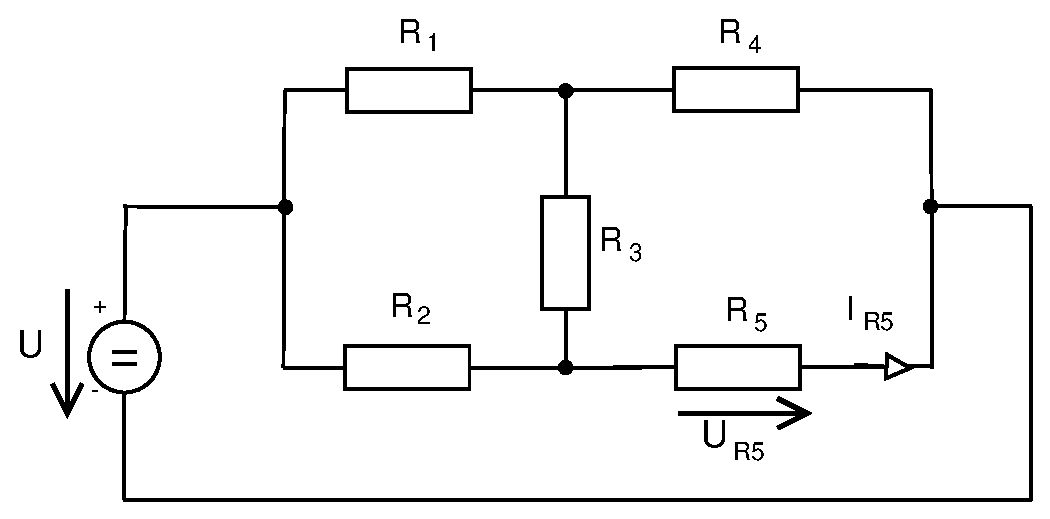
\includegraphics[height=4.5cm]{img/Pr2_2012.eps}
		\label{fig:pr2_obvod}
	\end{minipage}
	\begin{minipage}[c]{0.25\textwidth}
		$U = 250 V$ \\
		$R_{1} = 335 \Omega$ \\
		$R_{2} = 625 \Omega$ \\
		$R_{3} = 245 \Omega$ \\
		$R_{4} = 250 \Omega$ \\
		$R_{5} = 180 \Omega$ \\
		\\
		$U_{R_{5}} = ? V$ \\
		$I_{R_{5}} = ? A$ \\
	\end{minipage}
	\\

%===============================================================================

	\subsection*{Výpočet}
	
	Konverze trojúhelníku na hvězdu: \\
	
	\begin{tabbing}
		$ { \displaystyle R_{A} = \frac{R_{1} \times R_{2}} 
		{R_{1} + R_{2} + R_{3}} = 
		\frac{209375}{1205} = 173,755186722 \Omega}$ \\
		\\
		$ { \displaystyle R_{B} = \frac{R_{1} \times R_{3}} 
		{R_{1} + R_{2} + R_{3}} =  
		\frac{82075}{1205} = 68,112033195 \Omega}$ \\
		\\
		$ { \displaystyle R_{C} = \frac{R_{2} \times R_{3}} 
		{R_{1} + R_{2} + R_{3}} = 
		\frac{153125}{1205} = 127,074688797 \Omega}$ \\
		\\
	\end{tabbing}
	
	Vypočítání sériového zapojení: \\
	
	\begin{tabbing}
		$ { \displaystyle R_{B4} = R_{B} + R_{4} = 318,112033195 \Omega}$ \\
		\\
	\end{tabbing}
	
	Vypočítání $U_{0}$ a $R_{i}$: \\
	
	\begin{tabbing}
		$ { \displaystyle U_{0} = U \times \frac{R_{B4}}{R_{A}+R_{B4}} = 
		161,6859288 V}$\\
		\\
		$ { \displaystyle R_{i} = 
		\frac{R_{B4} \times R_{A}}{R_{B4}+R_{A}} + R_{C} = 
		239,449763793 \Omega}$ \\
		\\
	\end{tabbing}
	
	Vypočítání požadovaných hodnot:
	
	\begin{tabbing}
		$ { \displaystyle I_{R5} = \frac{U_{0}}{R_{i} + R_{5}} = 
		0,385471498 A}$ \\
	\end{tabbing}
	
	\begin{tabbing}
		$ { \displaystyle U_{R5} = R_{5} \times I_{R5} = 
		69,384869647 A}$ \\
	\end{tabbing}

	\newpage

%%%%%%%%%%%%%%%%%%%%%%%%%%%%%%%%%%%%%%%%%%%%%%%%%%%%%%%%%%%%%%%%%%%%%%%%%%%%%%%%

	\section*{Příklad č. 3 [B]} \label{pr3}

%===============================================================================

	\subsection*{Zadání}

	Stanovte napětí $U_{R4}$ a proud $I_{R4}$. Použíjte metodu uzlových napětí
	($U_{A}$, $U_{B}$, $U_{C}$). \\
	\\
	\begin{minipage}[c]{0.5\textwidth}
		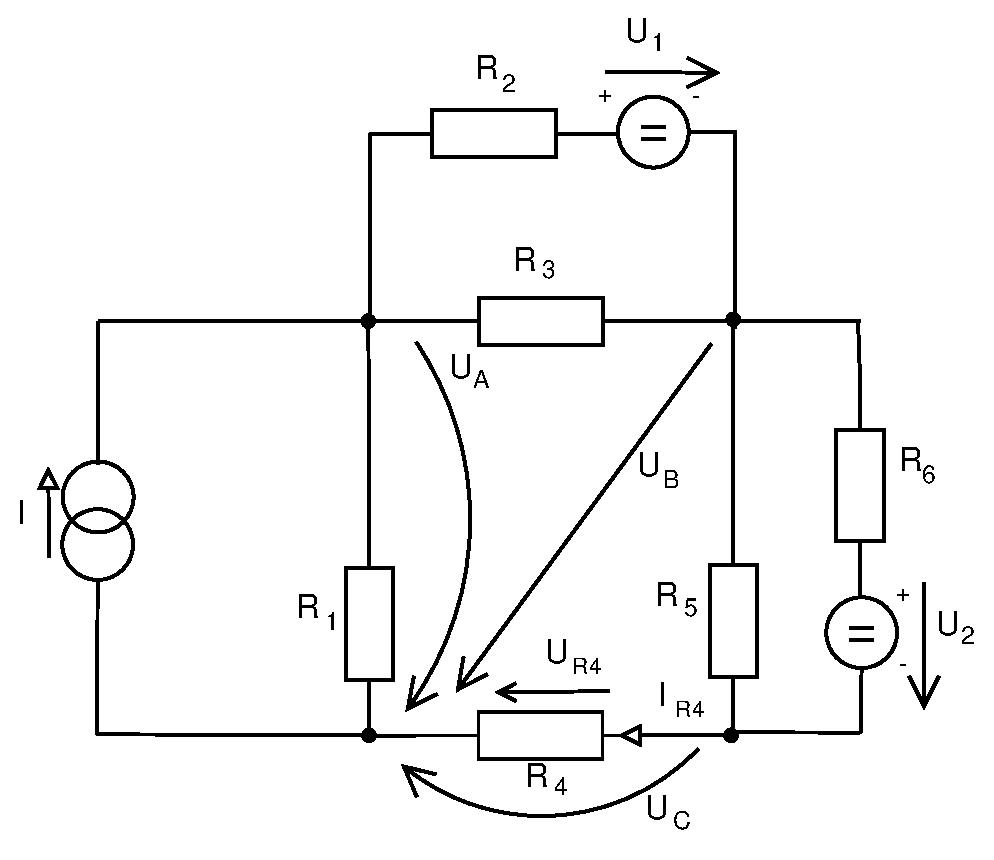
\includegraphics[height=7cm]{img/Pr3_2012.eps}
		\label{fig:pr3_obvod}
	\end{minipage}
	\begin{minipage}[c]{0.25\textwidth}
		$U_{1} = 150 V$ \\
		$U_{2} = 70 V$ \\
		$I = 0,8 A$ \\
		$R_{1} = 490 \Omega$ \\
		$R_{2} = 450 \Omega$ \\
		$R_{3} = 610 \Omega$ \\
		$R_{4} = 340 \Omega$ \\
		$R_{5} = 340 \Omega$ \\
		$R_{6} = 270 \Omega$ \\
		\\
		$U_{R4} = ? V$ \\
		$I_{R4} = ? A$
	\end{minipage}
	\\

%===============================================================================

	\subsection*{Výpočet}

	\quad Stanovení rovnic jednotlivých uzlů:
	
	\begin{tabbing}
		A: $I - I_{R1} + I_{R2} - I_{R3} = 0$ \\
		B: $I_{R3} - I_{R2} + I_{R6} - I_{R5} = 0$ \\
		C: $I_{R5} - I_{R6} - I_{R4} = 0$
	\end{tabbing}
	
	Vyjádření jednotlivých proudů:
	
	\begin{tabbing}
		$I_{R1}: I_{R1} \times R_{1} - U_{A} = 0$ \\
		$I_{R2}: I_{R2} \times R_{2} - U_{1} - U_{B} + U_{A} = 0$ \\
		$I_{R3}: I_{R3} \times R_{3} + U_{B} - U_{A} = 0$ \\
		$I_{R4}: I_{R4} \times R_{4} - U_{C} = 0$ \\
		$I_{R5}: I_{R5} \times R_{5} + U_{C} - U_{B} = 0$ \\
		$I_{R6}: I_{R6} \times R_{6} - U_{2} + U_{B} - U_{C} = 0$ \\
		\\
		${ \displaystyle I_{R1} = \frac{U_{A}}{R_{1}} }$ \quad
		${ \displaystyle I_{R2} = \frac{U_{1} + U_{B} - U_{A}}{R_{2}} }$ \quad
		${ \displaystyle I_{R3} = \frac{U_{A} - U_{B}}{R_{3}} }$ \quad
		${ \displaystyle I_{R4} = \frac{U_{C}}{R_{4}} }$ \quad
		${ \displaystyle I_{R5} = \frac{U_{B} - U_{C}}{R_{5}} }$ \\
		\\
		${ \displaystyle I_{R6} = \frac{U_{2} - U_{B} + U_{C}}{R_{6}} }$		
	\end{tabbing}
	\newpage
	Dosazení vyjádřených proudů do rovnic pro jednotlivé uzly:
	
	\begin{tabbing}
		${ \displaystyle I - 
		\frac{U_{A}}{R_{1}} + 
		\frac{U_{1} + U_{B} - U_{A}}{R_{2}} -
		\frac{U_{A} - U_{B}}{R_{3}} = 0 } $ \\ \\ \qquad $\Longrightarrow
		{ \displaystyle 0,8 - 
		\frac{U_{A}}{490} + 
		\frac{150 + U_{B} - U_{A}}{450} -
		\frac{U_{A} - U_{B}}{610} = 0 }$ \\
		\\ \\
		${ \displaystyle 
		\frac{U_{A} - U_{B}}{R_{3}} - 
		\frac{U_{1} + U_{B} - U_{A}}{R_{2}} + 
		\frac{U_{2} - U_{B} + U_{C}}{R_{6}} -
		\frac{U_{B} - U_{C}}{R_{5}} = 0 }$  \\ \\ \qquad $\Longrightarrow
		{ \displaystyle 
		\frac{U_{A} - U_{B}}{610} - 
		\frac{150 + U_{B} - U_{A}}{450} + 
		\frac{70 - U_{B} + U_{C}}{270} -
		\frac{U_{B} - U_{C}}{340} = 0 }$ \\
		\\ \\
		${ \displaystyle 
		\frac{U_{B} - U_{C}}{R_{5}} - 
		\frac{U_{2} - U_{B} + U_{C}}{R_{6}} -
		\frac{U_{C}}{R_{4}} = 0}$ \\ \\ \qquad $\Longrightarrow
		{ \displaystyle 
		\frac{U_{B} - U_{C}}{340} - 
		\frac{70 - U_{B} + U_{C}}{270} -
		\frac{U_{C}}{340} = 0}$ \\
		\\ \\
		$ U_{A} = 286,579 V $ \\
		$ U_{B} = 144,543 V $ \\
		$ U_{C} = 73,1494 V $ \\		
	\end{tabbing}
	
	Vypočítání požadovaného napětí $U_{R2}$ a proudu $I_{R2}$:
	
	\begin{tabbing}
		$U_{R4} = U_{C} = 73,1494 V$ \\
		\\
		${ \displaystyle I_{R4} = 
		\frac{U_{R4}}{R_{4}} =
		\frac{73,1494}{340} = 0,2151 A }$
	\end{tabbing}


	\newpage

%%%%%%%%%%%%%%%%%%%%%%%%%%%%%%%%%%%%%%%%%%%%%%%%%%%%%%%%%%%%%%%%%%%%%%%%%%%%%%%%

	\section*{Příklad č. 4 [A]} \label{pr4}

%===============================================================================

	\subsection*{Zadání}

	Pro napájecí napětí platí: $u = U \times \sin(2\pi ft)$.
	Ve vztahu pro napětí na cívce: \\ 
	$u_{L} = U_{L} \times \sin(2\pi ft + \varphi_{L})$ určtete $|U_{L}|$
	a $\varphi_{L}$.Použíjte metodu zjednodušování \\
	obvodu. \\
	
	\noindent Pozn: Pomocný "směr šipky napájecího zdroje platí pro \\
	speciální časový okamžik $(t = \frac{\pi}{2\omega} )$." \\
	\\
	
	\begin{minipage}[c]{0.6\textwidth}
		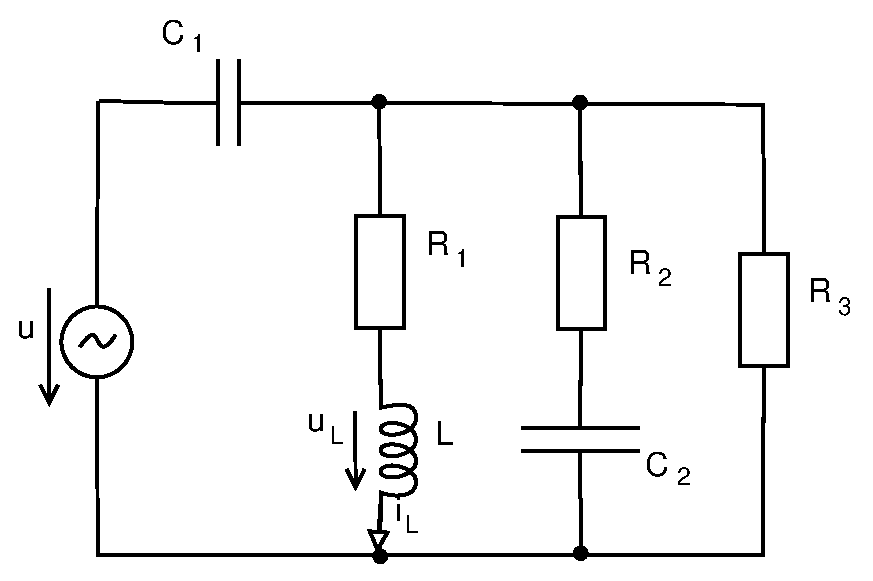
\includegraphics[height=5.5cm]{img/Pr4_2012.eps}
		\label{fig:pr4_obvod}
	\end{minipage}
	\begin{minipage}[c]{0.25\textwidth}
		$U_{1} = 45 V$ \\
		$R_{1} = 140 \Omega$ \\
		$R_{2} = 210 \Omega$ \\
		$R_{3} = 340 \Omega$ \\
		$L_{1} = 470 mH$ \\
		$C_{1} = 210 \mu F$ \\
		$C_{2} = 150 \mu F$ \\
		$f = 70 Hz$ \\
		\\
		$|U_{L}| = ? V$ \\
		$\varphi_{L} = ?$
	\end{minipage}
	\\

%===============================================================================

	\subsection*{Výpočet}

	$\omega = 2\pi f = 439,8229715 rad \times s^{-1}$
	
	\begin{tabbing}
		${ \displaystyle X_{C1} = 
		\frac{-1}{\omega \times C_{1}}j =
		\frac{-1}{439,8229715 \times 210 \times 10^{-6}}j = 
		-10,82686688j \Omega}$\\
		\\
		${ \displaystyle X_{C2} = 
		\frac{-1}{\omega \times C_{2}}j =
		\frac{-1}{439,8229715 \times 150 \times 10^{-6}}j = 
		-15,15761363j \Omega}$\\
		\\
		${ \displaystyle X_{L} = \omega \times L_{1}j = 
		439,8230 \times 470 \times 10^{-3} =
		149,5398j \Omega }$ \\
		\\
	\end{tabbing}
	
	\begin{tabbing}
		$ Z_{1} = R_{1} + X_{L} = 140 + 149,5398j \Omega $ \\
		\\
		$ Z_{2} = R_{2} + X_{C2} = 210 -15,1576j \Omega $ \\
		\\
		${ \displaystyle Z_{3} =
		\frac{ Z_{1} \times Z_{2} }{ Z_{1} + Z_{2} } =
		\frac{ 140 + 149,5398j \times 210 -15,1576j }
		     { 140 + 149,5398j + 210 -15,1576j } =
		     106,847 + 42,6371j \Omega }$\\
		\\
		${ \displaystyle Z_{3} =
		\frac{ Z_{1} \times Z_{2} }{ Z_{1} + Z_{2} } =
		\frac{ 140 + 149,5398j \times 210 -15,1576j }
		     { 140 + 149,5398j + 210 -15,1576j } =
		     106,847 + 42,6371j \Omega }$\\
		\\
		${ \displaystyle Z_{4} =
		\frac{ Z_{3} \times R_{3} }{ Z_{3} + R_{3} } =
		\frac{ (106,847 + 42,6371j) \times 340 }{ 106,847 + 42,6371j + 340 } =
		83,6326 + 24,4620j \Omega }$\\
		\\
	\end{tabbing}
	
	\begin{tabbing}
		$Z = Z_{4} + X_{C1} = 83,6326 + 24,4620j - 10,82686688j =
		83,6326 + 13,6351j \Omega $ \\
		\\
	\end{tabbing}
	
	\begin{tabbing}
		${ \displaystyle I = \frac{U}{Z} =
		\frac{45}{83,6326 + 13,6351j} = 0,524136 - 0,0854529j A }$ \\
		\\
		$U_{L} = I \times Z_{4} = 
		(0,5241 - 0,0855j) \times (83,6326 + 24,4620j) = 
		45,9233 + 5,6700j V$ \\
		\\
	\end{tabbing}
	
	\begin{tabbing}
		$|U_{L}| = \sqrt{45,9233^{2} + 5,6700^{2}} = 46,2720 V$\\
		\\
		$\varphi_{C1} = $
	\end{tabbing}

	\newpage
	
%%%%%%%%%%%%%%%%%%%%%%%%%%%%%%%%%%%%%%%%%%%%%%%%%%%%%%%%%%%%%%%%%%%%%%%%%%%%%%%%

	\section*{Příklad č. 5 [E]} \label{pr5}

%===============================================================================

	\subsection*{Zadání}

	Pro napájecí napětí platí: $u_{1} = U_{1} \times \sin(2\pi ft)$, 
	$u_{2} = U_{2} \times \sin(2\pi ft)$. 
	Ve vztahu \\ pro napětí na cívce $L_{1}$: 
	$u_{L_{1}} = U_{L_{1}} \times \sin(2\pi ft + \varphi_{L_{1}})$ určtete
	$|U_{L_{1}}|$ a $\varphi_{L}$. \\ Použíjte metodu smyčkových proudů. \\
	
	\noindent Pozn: Pomocný "směry šipek napájecích zdrojů platí pro časový 
	okamžik $(t = \frac{\pi}{2\omega} )$." \\
	\\
	
	\begin{minipage}[c]{0.6\textwidth}
		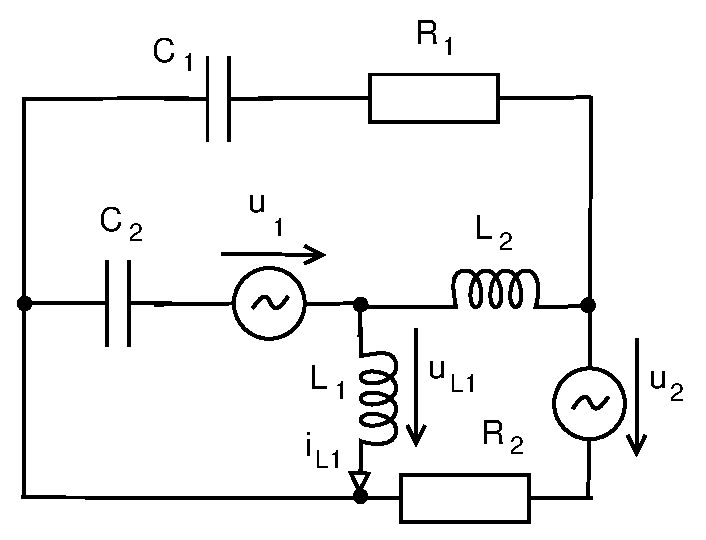
\includegraphics[height=5.5cm]{img/Pr5_2012.eps}
		\label{fig:pr5_obvod}
	\end{minipage}
	\begin{minipage}[c]{0.25\textwidth}
		$U_{1} = 50 V$ \\
		$U_{2} = 30 V$ \\
		$R_{1} = 145 \Omega$ \\
		$R_{2} = 135 \Omega$ \\
		$L_{1} = 130 mH$ \\
		$L_{2} = 60 mH$ \\
		$C_{1} = 100 \mu F$ \\
		$C_{2} = 65 \mu F$ \\
		$f = 90 Hz$ \\
		\\
		$|U_{L_{1}}| = ? V$ \\
		$\varphi_{L_{1}} = ?$
	\end{minipage}
	\\

%===============================================================================

	\subsection*{Výpočet}
	
	\begin{tabbing}
		
	\end{tabbing}
	
	\newpage
	
%%%%%%%%%%%%%%%%%%%%%%%%%%%%%%%%%%%%%%%%%%%%%%%%%%%%%%%%%%%%%%%%%%%%%%%%%%%%%%%%

	\section*{Příklad č. 6 [B]} \label{pr6}

%===============================================================================

	\subsection*{Zadání}

	Sestavte diferenciální rovnici popisující chodvání obvodu na obrázku, dále 
	ji \\ upravte dosazením hodnot parametrů. Vypočítejte analytické řešení
	$u_{C} = f(t)$. \\ Proveďte kontrolu výpočtu dosazením do sestavené
	diferenciální rovnice. \\
	\\
	
	\begin{minipage}[c]{0.4\textwidth}
		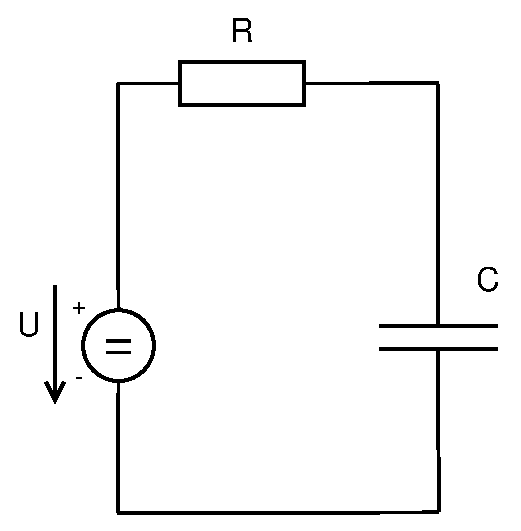
\includegraphics[height=5.5cm]{img/Pr6_2012.eps}
		\label{fig:pr6_obvod}
	\end{minipage}
	\begin{minipage}[c]{0.25\textwidth}
		$U = 6 V$ \\
		$C = 10 F$ \\
		$R = 20 \Omega $ \\
		$u_{C}(0) = 3 V$ \\
	\end{minipage}
	\\

%===============================================================================

	\subsection*{Výpočet}
	
	\begin{tabbing}
		${ \displaystyle U_{C}' = \frac{1}{C} \times I }$ \\
	\end{tabbing}
	
	Pro celkové napětí platí:
	
	\begin{tabbing}
		$U_{R} + U_{C} - U = 0$ \\
		\\
		$U = R \times I + U_{C}$ \\
		\\
		${ \displaystyle I = \frac{U - U_{C}}{R} }$ \\
		\\
	\end{tabbing}
	
	Dosazení zadané hodnoty:
	
	\begin{tabbing}
		${ \displaystyle U_{C}' = 
		\frac{1}{C} \times \frac{U - U_{C}}{R} =
		\frac{1 \times (6 - U_{C})}{10 \times 20} =
		\frac{(6 - U_{C})}{200}
		}$ \\
	\end{tabbing}
	
	Charakteristická rovnice:
	
	\begin{tabbing}
		$ 200 \times U_{C}' + U_{C} = 6$ \qquad $u_{c}(0) = 3$ \\
		\\
		$ 200 \lambda + 1 = 0$ \qquad \qquad \quad $\lambda = -0,005$\\
		\\
	\end{tabbing}
	
	Očekávané řešení:
	
	\begin{tabbing}
		$ U_{C}(t) = K (t) \times e^{ \lambda t} = K (t) \times e^{-0,005t} $\\
		\\
		$U_{C}' (t) = K' (t) \times e^{ \lambda t} +
		              K (t) \times \lambda \times e^{ \lambda t }$ \\
		\\
	\end{tabbing}
	
	Dosazení do charakteristické rovnice:
	
	\begin{tabbing}
		$ 200 (K' (t) \times e^{ \lambda t } + 
		  K (t) \times \lambda \times e^{ \lambda t} ) = 6 $ \\
		\\
		$ 200 K' (t) \times e^{ \lambda t} = 6 $ \\
		\\
		$ K' (t) \times e^{ \lambda t } = 0,03 $ \\
		\\
		$ { \displaystyle K' (t) = 
		\frac{0,03}{e^{ \lambda t }} = 
		\frac{0,03}{e^{-0.005t}} = 0,03e^{0,005t} }$ \\
		\\
	\end{tabbing}

	Integrace:
	
	\begin{tabbing}
		$ K (t) = 0,003 \times 
		\frac{1}{0,005} \times e^{-0,005t} = 6 \times e^{-0,005t} + q$ \\
		\\
	\end{tabbing}
	
	Dosazení do očekávaného řešení:
	
	\begin{tabbing}
		$ U_{C}(t) = (6 \times e^{0,005t} + q) \times e^{-0,005t} =
		6 + q \times e^{-0,005t}$ \\
		\\
	\end{tabbing}
	
	Nalezení $q$:
	
	\begin{tabbing}
		$ U_{C} (0) = 3 $ \\
		\\
		$ 3 = 6 + q \times e^{0} $ \\
		\\
		$ q = -3 $ \\
		\\
		$ U_{C} = 6 - 3 \times e^{-0,005t} $ \\
		\\ 
	\end{tabbing}
	
	Zkouška:
	
	\begin{tabbing}
		$ 200 \times U_{C}' + U_{C} = 6 $ \\
		\\
		$ 0 + 3 \times e^{-0,005t} + 6 -3 \times e^{-0,005t} = 6 $ \\
		\\
		6 = 6 \\
		\\		
	\end{tabbing}
	
	\newpage

%%%%%%%%%%%%%%%%%%%%%%%%%%%%%%%%%%%%%%%%%%%%%%%%%%%%%%%%%%%%%%%%%%%%%%%%%%%%%%%%

\end{document}
